\subsection{Functional Requirements}
\label{requirements:functional}
%Gerd
    \subsubsection{Entity Diagram}
    The following diagram shows all defined entities from the requirements above and their relations.
    As we can see a Task can either be modeled as a string or - if its a more complex task - modeled as an entirely new note.
    \begin{figure}[h]
    	% TODO remove the grey licensing text in the diagram by using the software with a valid license key
	    \centering
        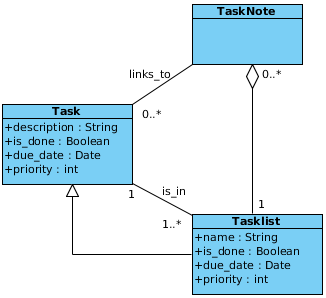
\includegraphics[width=0.5\textwidth]{graphics/entity_diagram.png}
        \caption{TaskList entities and relations}
        \label{entities_relations}
    \end{figure}
    
    This diagram does not define classes that must be implemented in software, but just the common entities



    \subsubsection{User Interface} %Jan
    \label{requirements:interfaces:user}

    \begin{requirement}{Create Task List}
      \desc{The user shall be able to create a new task list with a button or a shortcut text, like ``[]''. These lists expand automatically and contain individual tasks that can be marked as done.}
      \priority{1}
      \riskref{C}
    \end{requirement}

    \begin{requirement}{Edit Task List}
      \desc{The user can add, remove and change single task list items by directly editing the task list in the note itself.}
      \priority{1}
      \riskref{C}
    \end{requirement}

    \begin{requirement}{Priority}
      \desc{The user can optionally add and change priorities to individual tasks and task lists.}
      \priority{1}
      \riskref{H}
    \end{requirement}

    \begin{requirement}{Due date}
      \desc{The user can optionally add and change due dates to individual tasks and task lists, indicating when these should be finished. The system visualizes to the user when items are near or even over their due date.}
      \priority{1}
      \riskref{H}
    \end{requirement}

    \begin{requirement}{Create Subtasks}
      \desc{The user can optionally add subtasks to individual tasks. These subtasks are in principal linked notes, but can themselves contain tasks and task lists.}
      \priority{1}
      \riskref{H}
    \end{requirement}

    \begin{requirement}{Show / hide completed Tasks}
      \desc{The user has various possibilities to handle completed tasks. He can show them crossed out, he can hide them, and he can possibly show them after the completed tasks. }
      \priority{2}
      \riskref{M}
    \end{requirement}

    \begin{requirement}{Reorder Task Lists}
      \desc{The user has the possibility to order the task lists according to various criteria, like due date, priority, date added etc.}
      \priority{2}
      \riskref{L}
    \end{requirement}

	
	\subsubsection{Software Interfaces}
	\label{requirements:interfaces:software}
        %TODO => export (xml, evolution, tasque, ...)
        %     => Tomboy (save, ...)


	%\subsubsection{Communication Interfaces}
	%\label{requirements:interfaces:communication}

    \subsubsection{Supported Operating Systems}
    \label{requirements:os}
    \begin{requirement}{Platform independance}
      \desc{The Addin will work on any system with a working installation of Tomboy (as defined in ?)}
      \priority{2}
      \riskref{M}
%TODO: where is this defined, anyway? (Version etc)
    \end{requirement}

\subsection{Nonfunctional Requirements}
\label{requirements:nonfunctional}

    \subsubsection{Licensing Requirements}
    \label{requirements:nonfunctional_start}
    \label{requirements:license}
    %TODO: Not sure this is really necessary!
    \begin{requirement}{license compliance}
      \desc{The project will comply to any restrictions imposed by Tomboy/GNOME licensing.}
      \priority{2}
      \riskref{M}
    \end{requirement}


    \subsubsection{Language}
    \label{requirements:language}
    \begin{requirement}{Default language}
      \desc{All system messages, texts, log entries and help documentation must by default be in English.}
      \priority{1}
    \end{requirement}

   
    \begin{requirement}{Translations}
      \desc{The Addin will integrate the built in language support and will therefore enable anyone being capable of writing Tomboy/Gnome translations to add additional language translations to the project}
    \end{requirement}

    \begin{requirement}{Interface Requirement}
      \desc{insert description}
      \priority{1}
      \riskref{C}
    \end{requirement}


    %\subsection{Performance Requirements}
    %\label{requirements:performance}

    \subsubsection{Design Constraints}
    \label{requirements:constraints}

    \begin{requirement}{Standard compliance}
      \desc{The project will be seen as part of Tomboy and will therefore comply to any existing standards and regulations imposed by Tomboy itself or the GNOME project}
      \priority{2}
      \riskref{L}
    \end{requirement}

    % => modules (textbuffer, note gui, notes window gui)
    % I don't really see this being a design constraint (constraint = Auflage/Bedingung) - Gabriel

    \subsubsection{Quality Requirements}
    \label{requirements:quality}
    % => Bugs, unit tests

    %\subsection{Other Requirements}
    %\label{requirements:other}

    \label{requirements:nonfunctional_end}
